% =====================================================================
% Adaptive-QMIX manuscript (Paper 1) -- RESULT-INDEPENDENT DRAFT
%
% Status: draft of front matter, Introduction, Related Work, Problem
% Formulation and Methods, with Results/Discussion/Limitations skeletons.
% No empirical result of the adaptive study is reported in this file.
%
% Placeholders (search for them before submission):
%   TBD_AFTER_FINALISE_COARSE      Amendment-002 seal hashes (values exist;
%                                  to be copied from the sealed work orders)
%   TBD_AFTER_TIMING_VALIDATION    selected fixed-timing plan and the amended
%                                  baseline freeze (after fine search and
%                                  validation)
%   TBD_AFTER_LEARNER_TRAINING     official training outcomes
%   TBD_AFTER_LEARNER_VALIDATION   checkpoint selection, behaviour reports
%   TBD_AFTER_FINAL_EVALUATION     final held-out evaluation and statistics
%   OPTIONAL_ROBUSTNESS_AFTER_PRIMARY_GATE  high-demand slice (may be dropped)
%   % TODO-LITERATURE              citation still to be sourced and verified
%
% Source of truth for every methodological statement: the frozen
% implementation at commit 8c14f32988e92ddc6b1421d70258f5fbd2f2cc4d
% (config/adaptive_qmix/*.json, src/adaptive_qmix/**), Protocol Amendment
% 001 and Protocol Amendment 002 (revised). The historical DCHF manuscript
% (main.tex, supplementary.tex) is preserved unchanged and is not reused
% for any number.
% =====================================================================
\documentclass[review,12pt]{elsarticle}

\usepackage[utf8]{inputenc}
\usepackage[T1]{fontenc}
\usepackage{lmodern}
\usepackage{amsmath,amssymb,amsfonts,mathtools}
\usepackage{url}
\usepackage{graphicx}
\usepackage{booktabs}
\usepackage{multirow}
\usepackage{array}
\usepackage{float}
\usepackage{placeins}
\usepackage{setspace}
\usepackage{xcolor}
\usepackage{caption}
\usepackage[inline]{enumitem}
\usepackage{tabularx}
\usepackage{makecell}
\usepackage{tikz}
\usetikzlibrary{arrows.meta,positioning,calc,decorations.pathreplacing,fit}
\usepackage[colorlinks=true,linkcolor=blue,citecolor=blue,urlcolor=blue]{hyperref}
\pdfstringdefDisableCommands{%
  \def\corref#1{}%
  \def\cortext#1#2{}%
  \def\ead#1{}%
}

\newcolumntype{Y}{>{\raggedright\arraybackslash}X}
\newcolumntype{L}[1]{>{\raggedright\arraybackslash}p{#1}}
\renewcommand{\arraystretch}{1.15}
\setlength{\emergencystretch}{2em}
\onehalfspacing

% Visible markers for content that cannot be written before the data exist.
\newcommand{\TBD}[1]{\textcolor{red}{\texttt{\detokenize{#1}}}}
\newcommand{\Jp}{J_{\mathrm{primary}}}

\journal{Transportation Research Part C: Emerging Technologies}

\begin{document}

\hypersetup{pageanchor=false}
\begin{frontmatter}

% PROVISIONAL TITLE -- to be revisited after the final evaluation.
\title{Adaptive Cooperative Traffic Signal Control with QMIX under Short-Interval Green-Duration Decisions}

\author[inst1]{Mohamed Yassine Neifar\corref{cor1}}
\ead{yessine.neifar.imsil@isgis.usf.tn}
\cortext[cor1]{Corresponding author.}
\author[inst1]{Nadir Farhi}
\author[inst2]{Ahmed Frikha}
\address[inst1]{Universit\'e Gustave Eiffel, COSYS--GRETTIA,
14--20 Boulevard Newton, Cit\'e Descartes, Champs-sur-Marne,
F-77447 Marne-la-Vall\'ee Cedex 2, France}
\address[inst2]{Institut Sup\'erieur de Gestion Industrielle de Sfax,
OLID, University of Sfax, Route de l'A\'eroport km 4, BP 1099,
Sfax 3038, Tunisia}

\begin{abstract}
% ABSTRACT SKELETON. Design sentences are result-independent; every
% outcome sentence is a placeholder and must be written from the final
% evaluation only.
Multi-agent reinforcement learning (MARL) for traffic signal control is
often evaluated with a fixed cycle and fixed green splits, which leaves
the learned controller little genuine timing authority, and against
classical baselines that were not optimized. This paper evaluates
cooperative value-decomposition learning under genuine short-interval
green-duration authority. At two signalized intersections 300~m apart
(nominal spacing) under medium demand, each intersection decides every
5~s whether to extend the current green or to switch, with no fixed
cycle and no fixed adaptive green duration. QMIX is compared with VDN
and independent deep Q-learning under a matched implementation and a
matched interaction budget, and with classical baselines
optimized on dedicated design and validation traffic: an optimized
fixed-offset plan, an optimized fixed-timing plan whose cycle search
extends to the structural minimum cycle, and canonical Max Pressure.
The primary outcome is the mean scheduled waiting burden, which counts
waiting and insertion delay over every scheduled vehicle. Inference
uses ten independent training seeds crossed with ten held-out traffic
seeds, a paired crossed two-factor bootstrap, and a behavioural review
that precedes the performance comparison.
\TBD{TBD_AFTER_FINAL_EVALUATION}: primary outcome, cooperation
comparison, mixer comparison, Max Pressure comparison, and the
behavioural verdict.
\end{abstract}

\begin{keyword}
Adaptive traffic signal control \sep Multi-agent reinforcement learning
\sep QMIX \sep Value decomposition \sep Optimized fixed-time control
\sep Max Pressure \sep SUMO
\end{keyword}

\end{frontmatter}
\hypersetup{pageanchor=true}

% =====================================================================
\section{Introduction}
\label{sec:introduction}
% =====================================================================

Signal timing governs how green time is allocated among conflicting
movements, and at neighbouring intersections it also governs how
vehicles released at one junction meet the signal at the next. Classical
practice addresses both through cycle length, green splits and offsets,
chosen off-line for a design demand~\cite{webster1958,robertson1969transyt,little1981maxband,gartner1990multiband}.
Adaptive and actuated systems adjust these quantities in response to
detected traffic~\cite{hunt1981traffic,sims1980scoot}, and pressure-based
controllers choose phases from local queue information without a cycle
at all~\cite{varaiya2013max}. Reinforcement learning (RL), and for
multiple intersections multi-agent reinforcement learning (MARL), offers
a further alternative: a control policy learned by interaction with a
simulator~\cite{wei2018intellilight,chu2019multi,noaeen2022reinforcement}.

Whether such a policy can do anything a well-tuned classical plan
cannot depends first on what the policy is allowed to decide. If the
cycle length and green durations are fixed and the learned controller
only chooses which phase receives priority, or when an otherwise fixed
plan is shifted, then its authority over the timing of service is small
and the question \emph{what is the learner optimizing?} has a narrow
answer. A learned controller evaluated in that setting can show, at
most, how well it exploits the limited freedom it was given. This study
was designed around the opposite choice. Each intersection decides every
5~s whether to extend its current green or to switch to the conflicting
phase, so green durations, the realized cycle and the relative timing
of the two intersections all become outcomes of the policy rather than
parameters imposed on it.

The value of learning also depends on the reference it is measured
against. Network-level RL studies frequently compare against fixed-time
or other non-optimized controllers, so a reported improvement may
reflect the weakness of the reference as much as the quality of the
learned
policy~\cite{noaeen2022reinforcement}. A well-optimized pretimed plan
already captures a large share of the benefit available on a short
corridor under steady demand, and an adaptive pressure controller is a
strong non-learning alternative~\cite{varaiya2013max,levin2020max}. The
present study therefore optimizes its classical baselines on dedicated
design traffic, selects them on separate validation traffic, and freezes
them before any official learner is evaluated. When the optimized
fixed-timing search placed all of its best candidates on the lower
bound of the preregistered cycle range, the search was extended by a
documented protocol amendment rather than by a post-hoc argument, down
to the structural minimum cycle admitted by the classical plan rules
(Section~\ref{subsec:baseline_search}).

Finally, cooperative MARL claims require evidence that cooperation
matters. QMIX~\cite{Rashid2018} factorizes a joint action value into
per-agent utilities through a monotonic, state-conditioned mixing
network, trained centrally and executed without communication. Whether
this is useful at two intersections is an empirical question: an
additive factorization (VDN)~\cite{sunehag2017value} may suffice, and
independent learners sharing the same team reward may perform as well.
Learned controllers are also sensitive to the random seed of training,
so a single trained policy evaluated on many traffic realizations
measures robustness to traffic, not reliability of the training
procedure. This study uses ten independent training seeds per learned
method, crossed with ten held-out traffic seeds.

The paper addresses four research questions for a two-intersection
arterial with 300~m nominal spacing under medium, steady demand:
\begin{enumerate}[label=\textbf{RQ\arabic*.}, leftmargin=1.5cm]
\item Under short-interval green-duration authority, does QMIX reduce
the mean scheduled waiting burden relative to an optimized fixed-timing
plan selected under a preregistered design--validation protocol?
\item Does cooperative value decomposition improve on independent
learners that share the same reward, observation, architecture and
budget (QMIX versus IDQN), and does the monotonic mixer improve on
additive decomposition (QMIX versus VDN)?
\item How does QMIX compare with canonical operational Max Pressure, and
with a pressure rule executed under the same 5~s decision authority as
QMIX?
\item What signal behaviour does the learned policy produce---green
durations, switching burden, service deprivation, realized cycles and
inter-intersection timing---and does any coordination between the two
intersections emerge from the shared delay reward?
\end{enumerate}

The contributions are methodological as well as empirical:
\begin{itemize}
\item A controller formulation in which learned agents hold genuine
short-interval authority over green durations and phase sequencing,
with the temporal granularity of that authority stated exactly
(Section~\ref{subsec:executor}).
\item A comparator set in which every classical baseline is optimized
and selected on traffic disjoint from the final evaluation, including a
fixed-timing search whose cycle range was extended by preregistered
amendment to the structural minimum, and whose candidates are
identified by the signal plan actually executed rather than by
parameter labels.
\item An inferential design with independent training seeds as the unit
of learning variability, a crossed paired bootstrap, preregistered
decision rules without post-hoc effect-size thresholds, and a
behavioural gate that is applied before the performance comparison.
\item \TBD{TBD_AFTER_FINAL_EVALUATION}: empirical contribution, stated
according to the precommitted interpretation that applies
(Section~\ref{subsec:decision_rules}).
\end{itemize}

The scope is deliberately narrow: two intersections, one spacing, one
steady demand level, through movements only. The aim is to establish
what adaptive 5~s authority combined with cooperative learning buys in
a controlled setting before larger networks, other spacings or dynamic
demand are considered.

% =====================================================================
\section{Related work}
\label{sec:related}
% =====================================================================

\subsection{Classical signal timing and coordination}
\label{subsec:lit_classical}

Pretimed control assigns each phase a fixed green within a common cycle.
Webster's analysis of isolated signals established the classical
relationship between cycle length, lost time and delay, and remains the
reference point for cycle and split selection~\cite{webster1958}.
Arterial coordination adds offsets between neighbouring signals so that
platoons released upstream meet green downstream; TRANSYT optimizes
cycle, splits and offsets against a network delay model~\cite{robertson1969transyt},
while MAXBAND and MULTIBAND maximize progression
bandwidth~\cite{little1981maxband,gartner1990multiband,jingquanli2014}.
Because these methods optimize the same quantities a learned timing
controller would otherwise have to discover, a well-optimized pretimed
plan is a demanding reference. The present study does not assume any of
these models; it searches the pretimed plan space directly in the same
simulator and on the same traffic families used to evaluate the
learned controllers (Section~\ref{subsec:baseline_search}).
% TODO-LITERATURE: signal timing manual / HCM reference for pedestrian and
% operational minimum greens (for the deployability discussion only).

\subsection{Actuated, adaptive and pressure-based control}
\label{subsec:lit_adaptive}

Actuated control extends or terminates greens from detector calls, and
adaptive systems such as SCOOT~\cite{hunt1981traffic} and
SCATS~\cite{sims1980scoot} adjust cycles, splits and offsets
incrementally at network level. Their advantage over fixed-time control
narrows when the fixed-time plan is itself well
optimized~\cite{cameronkergaye2010}. Max Pressure selects, at each
intersection, the phase with the largest difference between upstream
and downstream vehicle counts over the movements it serves. Under its
stated network and demand assumptions it has a maximum-stability
property~\cite{varaiya2013max}; that property concerns throughput
feasibility, not delay minimization or progression, and practical phase
constraints such as minimum greens and cyclical phase structures require
modified formulations~\cite{levin2020max}. Progression-aware
variants exist~\cite{ahmed2025cmp}. The present study uses the
standard acyclic, decentralized formulation with an operational minimum
green as a transparent, reproducible non-learning adaptive reference,
and claims no stability property for its finite two-phase
implementation.

\subsection{Reinforcement learning for signal control and control authority}
\label{subsec:lit_rl}

Deep RL controllers learn a mapping from traffic state to signal action
by interaction with a simulator~\cite{Mnih2015,wei2018intellilight,samaheltantawy2014}.
Designs differ in state representation, reward and, less often
discussed, action space. Common action spaces select the next phase at a
fixed decision interval, decide whether to keep or change the current
phase, or adjust the durations or offsets of an otherwise cyclic
plan~\cite{noaeen2022reinforcement}.
% TODO-LITERATURE: a survey or benchmark paper that explicitly classifies
% RL signal-control action spaces (phase selection / keep-or-switch /
% phase-duration / cycle-based) -- needed to support this sentence
% precisely.
These choices determine the controller's temporal authority. A
keep-or-switch decision at a short interval, as used here, gives the
controller control over green durations and phase sequencing at the
resolution of the decision interval, but it also allows very short
greens and frequent switching, whose lost time and operational
acceptability must then be measured rather than assumed away.
% TODO-LITERATURE: prior reports of rapid switching / very short greens
% ("flickering") in RL signal control, and of minimum-green wrappers.
PressLight connects the RL reward to the Max Pressure
objective~\cite{wei2019presslight}, and decentralized designs scale to
many intersections~\cite{chen2020toward}; standardized benchmarks and
platforms have been proposed to make such comparisons
reproducible~\cite{ault2021reinforcement,mei2024libsignal,bokade2025pytsc}.

\subsection{Cooperative MARL and value decomposition}
\label{subsec:lit_marl}

When several intersections share a reward, independent learners face
a non-stationary problem and cannot attribute the joint outcome to their
own actions~\cite{foerster2018counterfactual}.
% TODO-LITERATURE: independent Q-learning (Tan, 1993) and independent deep
% Q-networks (Tampuu et al., 2017).
Centralized training with decentralized execution addresses this by
using global information only during training. Value-decomposition
methods factor the joint action value into per-agent utilities so that
greedy local action selection is consistent with the joint greedy
action: VDN uses a sum~\cite{sunehag2017value}, and QMIX a monotonic
mixing network whose weights are generated from the global
state~\cite{Rashid2018}. Later methods relax monotonicity at the cost of
more complex optimization~\cite{son2019qtran,rashid2020weighted,wang2021qplex}.
In traffic networks, cooperative MARL has been applied to large
grids~\cite{chu2019multi} and to corridors and networks with a variety
of coordination mechanisms~\cite{zhang2022distributed,kolat2023multi,jia2025multi},
and some work asks directly whether cooperation is always
beneficial~\cite{ren2025cooperative}. Few of these studies isolate the
contribution of the mixer by comparing QMIX, VDN and independent
learners under a matched implementation, matched initialization and a
matched interaction budget, as done here.

\subsection{Benchmarking and evaluation practice}
\label{subsec:lit_benchmarking}

Two evaluation practices limit what many RL signal-control results can
support. First, baselines are frequently fixed-time or otherwise
non-optimized~\cite{noaeen2022reinforcement}, and a reported margin
may then reflect the weakness of the reference.
% TODO-LITERATURE: a study showing RL margins shrinking against a tuned
% fixed-time or actuated reference (chenouyang2024 was used for this in
% the DCHF draft but its content has not been re-verified).
Second, learned controllers are often
reported from a single training run, evaluated on several traffic
realizations; this measures robustness to traffic, not the variability
of the learning procedure.
% TODO-LITERATURE: RL reproducibility and seed-variability literature
% (e.g., Henderson et al., 2018; Agarwal et al., 2021) -- verify and add.
A further, less visible issue concerns the outcome metric: measures
computed only over vehicles that entered the network can favour a
controller that delays insertion. The present design addresses the
three issues respectively with baselines optimized on disjoint design
and validation traffic, ten independent training seeds per learned
method, and a primary outcome over the full scheduled population that
counts insertion delay (Section~\ref{subsec:outcome}).

\subsection{Positioning}
\label{subsec:positioning}

The study does not propose a new learning algorithm. It asks a narrower
question that existing evaluations rarely answer cleanly: when a
cooperative value-decomposition learner is given genuine short-interval
authority over green durations at two neighbouring intersections, does
it outperform strong, independently optimized classical baselines, does
cooperation contribute beyond independent learning, and what signal
behaviour does it produce? The answer is sought under preregistered
decision rules, including the possibility that the optimized classical
plan or Max Pressure remains the stronger controller.

% =====================================================================
\section{Problem formulation}
\label{sec:problem}
% =====================================================================

\subsection{Corridor, demand and simulation environment}
\label{subsec:environment}

The study network is a two-intersection arterial modelled in
SUMO~\cite{Lopez2018} and controlled through TraCI
(Figure~\ref{fig:corridor}). Intersections J1 and J2 are separated by a
nominal junction spacing of $d=300$~m, which is the experimental design
factor. Because junction geometry occupies part of that distance, the
simulated central link between the two stop lines is a 279.2~m lane in
each direction; any travel-time or progression computation in this
paper uses the simulated lane length, not the nominal spacing. Every
approach has two lanes. Main-corridor approaches upstream of J1 and
downstream of J2 are 289.6~m lanes and the four side approaches are
189.6~m lanes. All routes are through movements, so each intersection
has two conflicting phases: H (main corridor) and V (side street).

Each episode schedules exactly 2{,}800 vehicles over the demand window
$[0,3600)$~s: 900 eastbound and 700 westbound on the main corridor, and
300 on each of the four side approaches. Within each stream the
departure seconds are drawn independently and uniformly over the
window, so the stream totals are fixed and the arrival pattern is a
conditioned homogeneous process with one-second resolution. Each
manifest is generated deterministically from its traffic family, seed
and index (Section~\ref{subsec:seeds}), and the per-episode SUMO seed is
derived from the same identifiers. A single passenger-car type is used
(length 5.0~m, minimum gap 2.5~m, maximum speed 13.89~m/s,
acceleration 2.6~m/s$^2$, deceleration 4.5~m/s$^2$, driver imperfection
$\sigma=0.5$ in SUMO's default car-following model).
% TODO-LITERATURE: Krauss car-following model reference (SUMO default).
Vehicles depart at maximum speed on the first free lane.

No capacity or saturation-flow value is assumed in this paper: the
operating point is characterized by the simulated outcomes themselves,
and no volume-to-capacity ratio is reported that would depend on an
unmeasured saturation flow.

\begin{figure}[!htbp]
\centering
\resizebox{0.95\textwidth}{!}{%
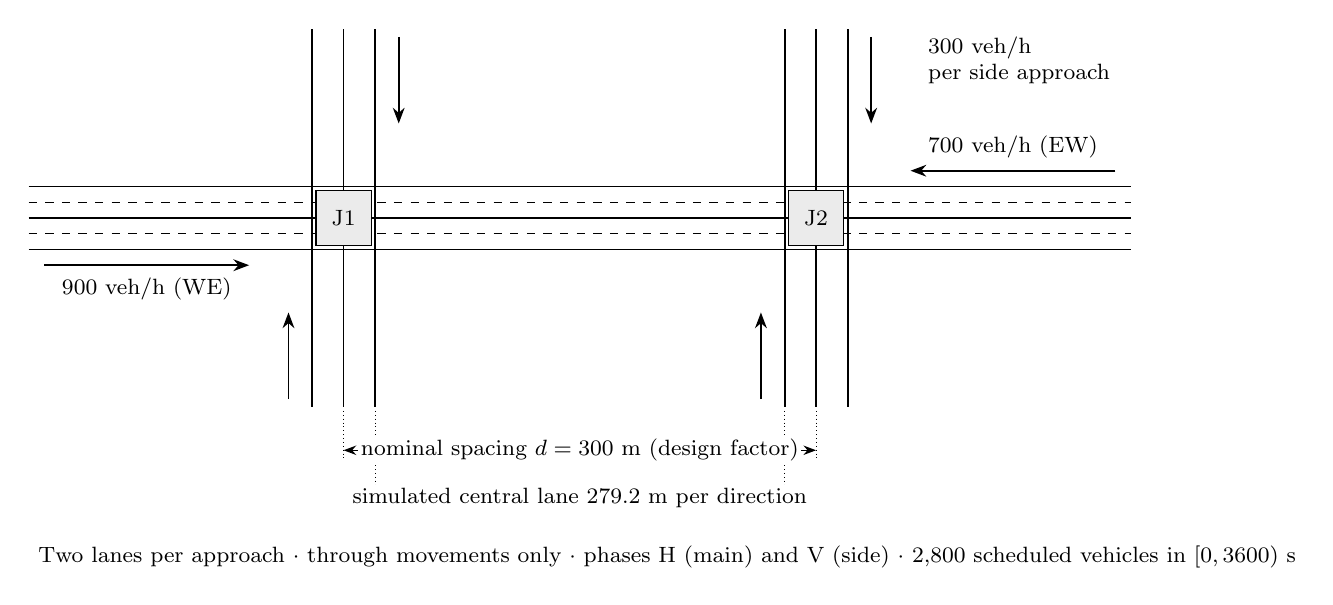
\begin{tikzpicture}[
  font=\footnotesize,
  road/.style={line width=0.7pt},
  lane/.style={dashed, line width=0.35pt},
  flow/.style={-{Stealth[length=2mm]}, line width=0.6pt},
  dim/.style={{Stealth[length=1.6mm]}-{Stealth[length=1.6mm]}, line width=0.45pt},
  jn/.style={draw, fill=black!8, minimum size=7mm, inner sep=0pt},
]
% main corridor
\draw[road] (-1.0, 0.40) -- (13.0, 0.40);
\draw[road] (-1.0,-0.40) -- (13.0,-0.40);
\draw[lane] (-1.0, 0.20) -- (13.0, 0.20);
\draw[lane] (-1.0,-0.20) -- (13.0,-0.20);
\draw[line width=0.5pt] (-1.0,0) -- (13.0,0);
% side streets
\foreach \x in {3.0,9.0}{
  \draw[road] (\x-0.40,-2.4) -- (\x-0.40,2.4);
  \draw[road] (\x+0.40,-2.4) -- (\x+0.40,2.4);
  \draw[line width=0.5pt] (\x,-2.4) -- (\x,2.4);
}
\node[jn] (J1) at (3.0,0) {J1};
\node[jn] (J2) at (9.0,0) {J2};
% flows
\draw[flow] (-0.8,-0.60) -- (1.8,-0.60) node[midway,below=1pt]{900 veh/h (WE)};
\draw[flow] (12.8,0.60) -- (10.2,0.60) node[midway,above=1pt]{700 veh/h (EW)};
\draw[flow] (3.7,2.3) -- (3.7,1.2);
\draw[flow] (2.3,-2.3) -- (2.3,-1.2);
\draw[flow] (9.7,2.3) -- (9.7,1.2);
\draw[flow] (8.3,-2.3) -- (8.3,-1.2);
\node[align=left, anchor=west] at (10.3,2.0) {300 veh/h\\per side approach};
% dimensions
\draw[densely dotted] (3.0,-2.45) -- (3.0,-3.05);
\draw[densely dotted] (9.0,-2.45) -- (9.0,-3.05);
\draw[densely dotted] (3.4,-2.45) -- (3.4,-3.65);
\draw[densely dotted] (8.6,-2.45) -- (8.6,-3.65);
\draw[dim] (3.0,-2.95) -- (9.0,-2.95) node[midway,fill=white,inner sep=1pt]
  {nominal spacing $d=300$~m (design factor)};
\draw[dim] (3.4,-3.55) -- (8.6,-3.55) node[midway,fill=white,inner sep=1pt]
  {simulated central lane 279.2~m per direction};
\node[anchor=west, align=left] at (-1.0,-4.3)
  {Two lanes per approach $\cdot$ through movements only $\cdot$ phases H (main) and V (side)
   $\cdot$ 2{,}800 scheduled vehicles in $[0,3600)$~s};
\end{tikzpicture}}
\caption{Study corridor. The nominal spacing of 300~m is the experimental
design factor; the simulated link between stop lines is 279.2~m and is
used for any travel-time computation. Demand is fixed per stream and per
episode; departure times are random within the one-hour demand window.}
\label{fig:corridor}
\end{figure}

\subsection{Adaptive signal-control formulation and temporal authority}
\label{subsec:executor}

Both intersections are controlled on a single, globally synchronized
decision clock with interval $\Delta t=5$~s. At each decision instant
$t_k=5k$~s, $k=0,1,\dots$, intersection $i\in\{\mathrm{J1},\mathrm{J2}\}$
selects an action $a_i(t_k)\in\{\textsc{extend},\textsc{switch}\}$:
\begin{itemize}
\item \textsc{extend} keeps the current green for the next 5~s;
\item \textsc{switch} fills the next 5~s with 3~s of yellow for the
current phase followed by 2~s of green for the conflicting phase.
\end{itemize}
Both actions last exactly 5~s, so every joint transition spans 5~s of
simulated time. The executor imposes no cycle length, no offset, no
fixed green duration, no maximum green and no minimum green beyond what
the decision grid itself implies. That grid has consequences that must
be stated precisely rather than summarized as ``no minimum green''
(Figure~\ref{fig:executor}):
\begin{enumerate}[label=(\roman*)]
\item \emph{Greens entered by switching.} A green that begins with the
2~s segment of a \textsc{switch} and is then extended $k\geq 0$ times
lasts $2+5k$~s. The shortest possible such green is 2~s, which occurs
when a \textsc{switch} is immediately followed by another
\textsc{switch}.
\item \emph{Initial green.} At $t=0$ both intersections show H green
with zero elapsed green and no warm-up period, and the first joint
decision is taken at $t=0$. The initial H green therefore lasts $5k$~s
for some $k\geq 0$; $k=0$ means that the first decision is
\textsc{switch} and the yellow begins at $t=0$.
\item \emph{Clearance interval.} Every change of phase is preceded by
exactly 3~s of yellow; there is no separate all-red interval.
\item \emph{Realized cycles.} A full H--V sequence composed of two greens
entered by switching lasts $(2+5k_H)+3+(2+5k_V)+3=10+5(k_H+k_V)$~s, so
realized cycles are multiples of 5~s and at least 10~s long. They are
outcomes of the policy, not parameters.
\item \emph{Relative timing.} Because both intersections act on the same
clock, the time between a phase change at J1 and a phase change at J2 is
a multiple of 5~s. The learned controllers can therefore realize
inter-intersection timing relationships only at 5~s resolution, whereas
the pretimed baselines of Section~\ref{subsec:classical} realize offsets
at 1~s resolution.
\end{enumerate}
These properties define the control authority under evaluation. They
also mean that frequent switching is possible and costs 3~s of yellow
per switch; the switching burden and the distribution of realized green
durations are therefore reported for every adaptive policy
(Section~\ref{subsec:behaviour}). A minimum-green wrapper would define a
different controller and is not part of the primary specification.

\begin{figure}[!htbp]
\centering
\resizebox{0.95\textwidth}{!}{%
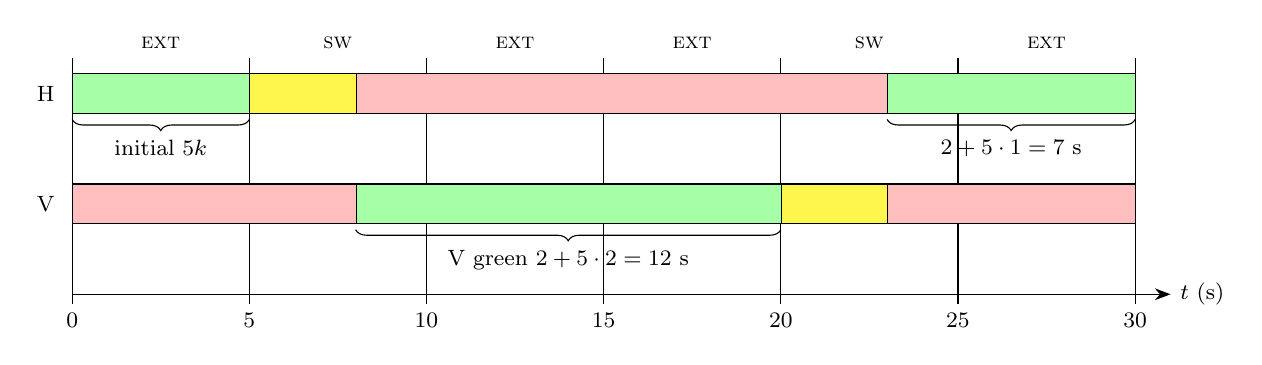
\begin{tikzpicture}[
  font=\footnotesize,
  sgreen/.style={draw, fill=green!35, minimum height=5mm, inner sep=0pt},
  sred/.style={draw, fill=red!25, minimum height=5mm, inner sep=0pt},
  syellow/.style={draw, fill=yellow!70, minimum height=5mm, inner sep=0pt},
  tick/.style={line width=0.4pt},
]
\def\u{0.45} % 1 s
\def\yH{1.95}
\def\yV{0.55}
% time axis and decision ticks
\draw[-{Stealth[length=2mm]}] (0,-0.6) -- (31*\u,-0.6) node[right]{$t$ (s)};
\foreach \k in {0,...,6}{
  \draw[tick] (5*\k*\u,-0.72) -- (5*\k*\u,2.4);
  \node[below] at (5*\k*\u,-0.72) {\pgfmathparse{int(5*\k)}\pgfmathresult};
}
\node[anchor=east] at (-0.1,\yH) {H};
\node[anchor=east] at (-0.1,\yV) {V};
% actions at t = 0,5,...,25: EXTEND, SWITCH, EXTEND, EXTEND, SWITCH, EXTEND
\foreach \c/\a in {2.5/ext,7.5/sw,12.5/ext,17.5/ext,22.5/sw,27.5/ext}{
  \node[above] at (\c*\u,2.4) {\textsc{\a}};
}
% H signal row
\node[sgreen, minimum width=5*\u cm, anchor=west] at (0,\yH) {};
\node[syellow, minimum width=3*\u cm, anchor=west] at (5*\u,\yH) {};
\node[sred, minimum width=15*\u cm, anchor=west] at (8*\u,\yH) {};
\node[sgreen, minimum width=7*\u cm, anchor=west] at (23*\u,\yH) {};
% V signal row
\node[sred, minimum width=8*\u cm, anchor=west] at (0,\yV) {};
\node[sgreen, minimum width=12*\u cm, anchor=west] at (8*\u,\yV) {};
\node[syellow, minimum width=3*\u cm, anchor=west] at (20*\u,\yV) {};
\node[sred, minimum width=7*\u cm, anchor=west] at (23*\u,\yV) {};
% annotations (below each row)
\draw[decorate,decoration={brace,amplitude=4pt,mirror}]
  (0,1.62) -- (5*\u,1.62) node[midway,below=4pt]{initial $5k$};
\draw[decorate,decoration={brace,amplitude=4pt,mirror}]
  (23*\u,1.62) -- (30*\u,1.62) node[midway,below=4pt]{$2+5\cdot1=7$~s};
\draw[decorate,decoration={brace,amplitude=4pt,mirror}]
  (8*\u,0.22) -- (20*\u,0.22) node[midway,below=4pt]{V green $2+5\cdot2=12$~s};
\end{tikzpicture}}
\caption{Executor semantics at one intersection (illustrative action
sequence, not a learned policy). Decisions occur every 5~s.
\textsc{extend} adds 5~s of the current green; \textsc{switch} gives 3~s
of yellow and 2~s of the new green. A green entered by switching lasts
$2+5k$~s; the initial green lasts $5k$~s; realized cycles are multiples
of 5~s. Both intersections share the same decision clock.}
\label{fig:executor}
\end{figure}

\subsection{Observations, actions, global state and reward}
\label{subsec:mdp}

\paragraph{Local observation}
Each agent observes an eight-dimensional vector computed at the decision
instant from its own intersection only
(Table~\ref{tab:observation}):
\begin{equation}
o_i=\bigl[\hat q_H,\ \hat q_V,\ p_i,\ \hat g_i,\ \hat\lambda_H,\ \hat\lambda_V,\
\widehat{\mathit{Occ}}_{H,\mathrm{out}},\ \widehat{\mathit{Occ}}_{V,\mathrm{out}}\bigr].
\label{eq:observation}
\end{equation}
$\hat q_H$ and $\hat q_V$ are the numbers of halting vehicles on the
four incoming lanes of each movement group, divided by 150 and 100
respectively and clipped to $[0,1]$. $p_i$ is the current logical
phase ($1$ for H, $0$ for V). $\hat g_i=g_i/(g_i+60)$ scales the elapsed
green $g_i$ in seconds. $\hat\lambda_m=\lambda_m/(\lambda_m+1)$ scales
the mean arrival rate $\lambda_m$ (veh/s) of new vehicles onto the
incoming lanes of movement group $m$ over the preceding 30~s. The last
two entries are the largest SUMO occupancy fraction among the outgoing
(receiving) lanes of each movement group. No offset, platoon position,
coordination phase or neighbouring action is observed.

\paragraph{Actions}
$a_i\in\{0,1\}$ with $0=\textsc{extend}$ and $1=\textsc{switch}$, as
defined in Section~\ref{subsec:executor}. The joint action space has
four elements.

\paragraph{Global state}
The state used by the QMIX mixer during training is the concatenation
of the two local observations, $s=[o_1,o_2]\in\mathbb{R}^{16}$. No
information outside the two observations is added, and no
communication between agents takes place at execution.

\paragraph{Reward}
All agents receive the same network reward for decision block $k$,
which covers the five simulated seconds $\tau$ of that block:
\begin{equation}
r_k=-\sum_{\tau\in k}\Bigl[N_{\text{stopped,active}}(\tau)
+N_{\text{pending,due}}(\tau)\Bigr],
\label{eq:reward}
\end{equation}
where $N_{\text{stopped,active}}(\tau)$ is the number of vehicles in the
network with speed at most 0.1~m/s at second $\tau$, and
$N_{\text{pending,due}}(\tau)$ is the number of vehicles whose scheduled
departure time has passed but which have not yet been inserted. The
reward is in vehicle-seconds and is not rescaled. It contains no offset,
platoon, green-wave, switching, minimum-green or fairness term: any
coordination between the intersections must arise from shared delay
pressure alone. Including insertion backlog in the reward, as in the
primary outcome below, removes the incentive to keep vehicles out of
the network.

\begin{table}[!htbp]
\centering
\caption{Local observation of agent $i$ (frozen specification).}
\label{tab:observation}
\small
\begin{tabularx}{\textwidth}{@{}lL{3.8cm}Y@{}}
\toprule
Feature & Raw quantity & Normalization \\
\midrule
$\hat q_H$ & halting vehicles, H incoming lanes (4) & $\min(1,q_H/150)$ \\
$\hat q_V$ & halting vehicles, V incoming lanes (4) & $\min(1,q_V/100)$ \\
$p_i$ & current logical phase & 1 if H, 0 if V \\
$\hat g_i$ & elapsed green $g_i$ (s) & $g_i/(g_i+60)$ \\
$\hat\lambda_H,\hat\lambda_V$ & new vehicles entering incoming lanes, mean over last 30~s (veh/s) & $\lambda/(\lambda+1)$ \\
$\widehat{\mathit{Occ}}_{H,\mathrm{out}},\widehat{\mathit{Occ}}_{V,\mathrm{out}}$ & SUMO lane occupancy of receiving lanes & maximum over the lanes, in $[0,1]$ \\
\bottomrule
\end{tabularx}
\end{table}

\subsection{Episodes, clearance and primary outcome}
\label{subsec:outcome}

An episode begins at $t=0$ with empty links and ends when every one of
the 2{,}800 scheduled vehicles has been inserted and has left the
network. Demand stops at 3{,}600~s but simulation continues until the
network clears. If the network has not cleared by 7{,}200~s the episode
ends with status \textsc{clearance\_failure}; such an episode has no
valid primary outcome (Section~\ref{subsec:validity}).

The primary outcome is the mean scheduled waiting burden
\begin{equation}
\Jp=\frac{1}{2800}\sum_{v=1}^{2800}\bigl(w_v+\delta_v\bigr),
\label{eq:jprimary}
\end{equation}
where $w_v$ is SUMO's trip waiting time of vehicle $v$ (time spent at
speed at most 0.1~m/s) and $\delta_v$ is its departure delay, the time
between its scheduled departure and its actual insertion.
% TODO-LITERATURE: SUMO documentation for tripinfo waitingTime and
% departDelay definitions.
The denominator is the full scheduled population, so a controller cannot
improve $\Jp$ by delaying insertion. $\Jp$ is defined only for episodes
that clear with every scheduled vehicle accounted for. It is the only
quantity used for the primary decision; it is not comparable with the
waiting measure of earlier work by the authors, which used a different
definition.

\subsection{Secondary outcomes}
\label{subsec:secondary}

The following outcomes are committed for reporting before any official
learner is evaluated. They describe the result but never replace $\Jp$
in the primary decision:
mean completed-vehicle time loss, mean travel time, mean number of
stops, number of completed vehicles, clearance status, 95th-percentile
and maximum queue, realized green-duration distribution including the
frequency and mass of 2~s greens, switch count and rate, yellow seconds
and yellow fraction of elapsed time, 95th-percentile and maximum service
deprivation, service frequency, phase green share, the emergent-cycle
distribution, and the coordination diagnostics of
Section~\ref{subsec:mechanism}.

% =====================================================================
\section{Controllers}
\label{sec:controllers}
% =====================================================================

Table~\ref{tab:controllers} lists every controller and its role. Seven
controllers are official comparators; one pressure rule is a diagnostic
only.

\begin{table}[!htbp]
\centering
\caption{Controllers and their methodological roles.}
\label{tab:controllers}
\small
\begin{tabularx}{\textwidth}{@{}L{3.3cm}L{4.4cm}Y@{}}
\toprule
Controller & Timing authority & Role \\
\midrule
QMIX & 5~s \textsc{extend}/\textsc{switch}, learned, monotonic mixer & Treatment. \\
VDN & same executor, additive decomposition & Mixer comparison (reported, not deciding). \\
IDQN & same executor, independent learners, shared reward & Cooperation comparison (deciding). \\
Optimized fixed timing & pretimed; cycle, split and offset searched & Primary classical comparator (deciding). \\
Optimized fixed offset & pretimed; $C=90$~s, equal greens, offset searched & Classical reference (reported). \\
Simultaneous fixed time & pretimed; $C=90$~s, equal greens, $\Delta=0$ & Uncoordinated reference (reported). \\
Canonical Max Pressure & acyclic, 1~s re-evaluation after a 10~s minimum green & Operational adaptive baseline (mandatory report, not a gate). \\
P5 (diagnostic) & pressure rule on the QMIX 5~s executor & Separates pressure logic from decision authority; not an official controller. \\
\bottomrule
\end{tabularx}
\end{table}

\subsection{Learned controllers: QMIX, VDN and IDQN}
\label{subsec:learners}

The three learned methods share every component except value
decomposition (Figure~\ref{fig:architecture}). Each intersection has its
own local Q-network with architecture
$8\rightarrow128\rightarrow128\rightarrow2$ and ReLU activations; weights
are not shared between the two agents. For a given training seed, the
two local networks are initialized identically across the three methods,
from random-number streams derived from the training seed and the agent
name, so that differences between methods at the same seed are not
differences in initialization. Execution is decentralized in all three
methods: each agent acts greedily on its own local Q-values.

\paragraph{QMIX} The joint value is
$Q_{\mathrm{tot}}(s,\mathbf a)=f_{\psi}\bigl(Q_1(o_1,a_1),Q_2(o_2,a_2);s\bigr)$,
where the mixing network $f_\psi$ has one hidden layer of 32 units with
ELU activation. Its weights are produced from the 16-dimensional state
by hypernetworks with 64 hidden units and are constrained to be
non-negative by an absolute value, which makes $Q_{\mathrm{tot}}$
monotonic in each local value; the biases, including a state-dependent
final bias with a 32-unit hidden layer, are unconstrained~\cite{Rashid2018}.

\paragraph{VDN} $Q_{\mathrm{tot}}(s,\mathbf a)=Q_1(o_1,a_1)+Q_2(o_2,a_2)$~\cite{sunehag2017value}.

\paragraph{IDQN} Each agent is trained on its own temporal-difference
error using its own local target, with the shared team reward of
Eq.~\eqref{eq:reward}; there is no mixer and no global state.
% TODO-LITERATURE: independent (deep) Q-learning references.

\paragraph{Learning update} All three methods use Double-DQN targets:
the next action of each agent is selected by its online network and
evaluated by its target network.
% TODO-LITERATURE: van Hasselt, Guez and Silver (2016), Double DQN.
With a decision block of $\Delta t_k$ seconds the discount is
$\gamma^{\Delta t_k/5}$ with $\gamma=0.99$ per 5~s; since every block
lasts 5~s this equals $0.99$. The bootstrap term is masked only when the
episode terminates by clearance. Truncation by the 7{,}200~s cap or by
the interaction budget does not mask it, because the state after a
truncation is not terminal. For QMIX and VDN the target is
\begin{equation}
y=r_k+\mathbb{1}[\neg\text{terminated}]\,\gamma^{\Delta t_k/5}\,
Q^{-}_{\mathrm{tot}}\bigl(s',\bar{\mathbf a}';\ s'\bigr),\qquad
\bar a'_i=\arg\max_{a}Q_i(o'_i,a),
\label{eq:target}
\end{equation}
with the target mixer $Q^{-}_{\mathrm{tot}}$ applied to target local
values; for IDQN the same target is formed per agent from its own target
local value. The loss is the Huber (smooth-$L_1$) loss with
$\beta=1$, averaged over the batch; for IDQN the two agents' losses are
summed.
% TODO-LITERATURE: Huber (1964) loss; Adam (Kingma and Ba, 2015).
Parameters are optimized with Adam at learning rate $5\times10^{-4}$.
Gradients are clipped to a global $L_2$ norm of 10 over all parameters
entering the cooperative loss (QMIX, VDN) and per agent for IDQN.
Target networks, including the target mixer, are hard-copied every 500
learner updates. Table~\ref{tab:hyperparameters} lists the frozen
training configuration.

\begin{figure}[!htbp]
\centering
\resizebox{0.95\textwidth}{!}{%
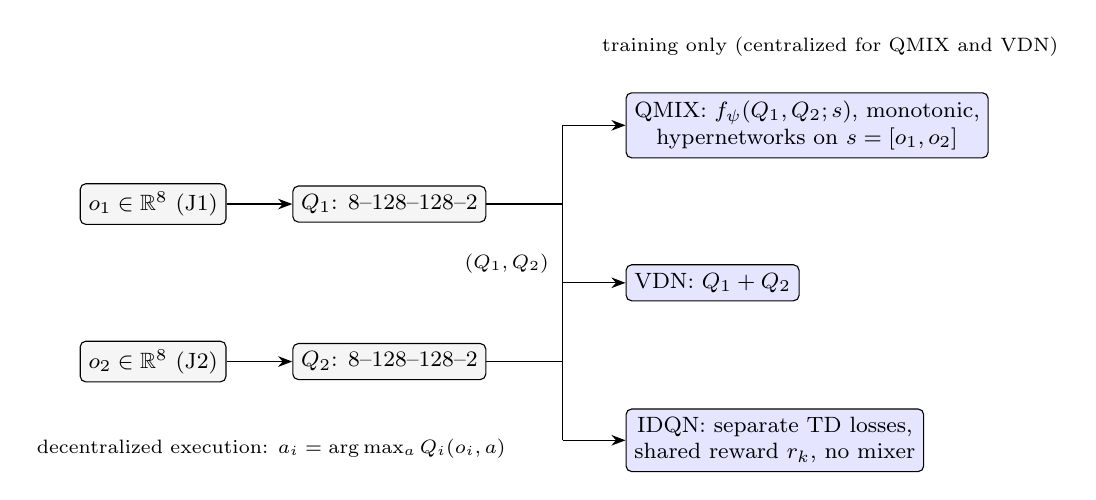
\begin{tikzpicture}[
  font=\footnotesize,
  box/.style={draw, rounded corners=2pt, align=center, inner sep=3pt, fill=black!4},
  mix/.style={draw, rounded corners=2pt, align=center, inner sep=3pt, fill=blue!10},
  ar/.style={-{Stealth[length=1.8mm]}, line width=0.5pt},
  lab/.style={font=\footnotesize\bfseries},
]
% local networks (identical for the three methods)
\node[box] (o1) at (0,2.2) {$o_1\in\mathbb R^8$ (J1)};
\node[box] (o2) at (0,0.2) {$o_2\in\mathbb R^8$ (J2)};
\node[box] (q1) at (3.0,2.2) {$Q_1$: 8--128--128--2};
\node[box] (q2) at (3.0,0.2) {$Q_2$: 8--128--128--2};
\draw[ar] (o1) -- (q1); \draw[ar] (o2) -- (q2);
\node[align=center, font=\scriptsize] at (1.5,-0.9) {decentralized execution:
$a_i=\arg\max_a Q_i(o_i,a)$};
% common connection carrying (Q_1, Q_2)
\draw[line width=0.5pt] (q1.east) -- (5.2,2.2);
\draw[line width=0.5pt] (q2.east) -- (5.2,0.2);
\draw[line width=0.5pt] (5.2,-0.8) -- (5.2,3.2);
\node[font=\scriptsize, anchor=south east] at (5.15,1.2) {$(Q_1,Q_2)$};
% training-time decompositions
\node[mix, anchor=west] (qm) at (6.0,3.2) {QMIX: $f_\psi(Q_1,Q_2;s)$, monotonic,\\hypernetworks on $s=[o_1,o_2]$};
\node[mix, anchor=west] (vd) at (6.0,1.2) {VDN: $Q_1+Q_2$};
\node[mix, anchor=west] (id) at (6.0,-0.8) {IDQN: separate TD losses,\\shared reward $r_k$, no mixer};
\draw[ar] (5.2,3.2) -- (qm.west);
\draw[ar] (5.2,1.2) -- (vd.west);
\draw[ar] (5.2,-0.8) -- (id.west);
\node[font=\scriptsize] at (8.6,4.2) {training only (centralized for QMIX and VDN)};
\end{tikzpicture}}
\caption{Matched learned controllers. The local networks, observation,
executor, reward, initialization, replay, exploration schedule and
interaction budget are identical; only the value decomposition used in
training differs. The global state used by the QMIX hypernetworks is
the concatenation of the two local observations.}
\label{fig:architecture}
\end{figure}

\begin{table}[!htbp]
\centering
\caption{Frozen learning configuration, identical for QMIX, VDN and IDQN
unless stated.}
\label{tab:hyperparameters}
\small
\begin{tabularx}{\textwidth}{@{}L{5.6cm}Y@{}}
\toprule
Item & Value \\
\midrule
Local network & 8--128--128--2, ReLU, separate weights per agent \\
QMIX mixer & 32 mixing units (ELU); hypernetworks with 64 hidden units; non-negative weights \\
Target & Double DQN; bootstrap masked only on clearance termination \\
Discount & $\gamma^{\Delta t/5}$, $\gamma=0.99$ per 5~s \\
Loss & Huber, $\beta=1$ \\
Optimizer & Adam, learning rate $5\times10^{-4}$ \\
Gradient clipping & global $L_2$ norm 10 (per agent for IDQN) \\
Replay buffer & 200{,}000 joint transitions; batch 256 \\
Warm-up & 5{,}000 transitions before the first update \\
Updates & one learner update per transition after warm-up \\
Target update & hard copy every 500 learner updates \\
Exploration & $\varepsilon$ linear from 1.0 to 0.05 over the first 250{,}000 transitions, then 0.05; independent draws per agent \\
Budget & 360{,}000 joint transitions; 355{,}000 learner updates \\
Checkpoints & 50k, 75k, 100k, \ldots, 350k (every 25k) and 360k transitions (14 in total) \\
Training seeds & 101--110 per method \\
Device & CPU; deterministic PyTorch algorithms enabled \\
\bottomrule
\end{tabularx}
\end{table}

\subsection{Classical comparators}
\label{subsec:classical}

All pretimed plans use two phases, H then V, each followed by a 3~s
yellow, so that $g_H+g_V+6=C$. Plans are executed at 1~s resolution.
J1 carries offset 0 and J2 carries offset $\Delta$, defined as the time
from the start of H green at J1 to the start of H green at J2, modulo
$C$. Both schedules run in periodic steady state from $t=0$, without a
start-up transient.

\paragraph{Simultaneous fixed time} $C=90$~s, $g_H=g_V=42$~s,
$\Delta=0$. This is an uncoordinated reference.

\paragraph{Optimized fixed offset} The simultaneous timing with $\Delta$
searched over all 90 integer values
(Section~\ref{subsec:baseline_search}). The plan selected on validation
traffic, $(C,f_H,\Delta)=(90~\mathrm{s},0.500,41~\mathrm{s})$, is used
unchanged throughout.
% VERIFY: copy from the offset_validation selected-plan artefact recorded
% in the amended freeze before submission.

\paragraph{Optimized fixed timing} Cycle, split and offset are searched
jointly (Section~\ref{subsec:baseline_search}). The selected plan is
\TBD{TBD_AFTER_TIMING_VALIDATION}.

\paragraph{Canonical Max Pressure} At each intersection independently,
the pressure of phase $p$ is
\begin{equation}
P_i(p,t)=\sum_{(l,m)\in\mathcal M_i(p)}\bigl[n_l(t)-n_m(t)\bigr],
\label{eq:pressure}
\end{equation}
where $\mathcal M_i(p)$ is the set of incoming--outgoing lane pairs of
the through movements served by $p$ and $n_l(t)$ is the number of
vehicles on lane $l$~\cite{varaiya2013max}. After a minimum green of
10~s, the pressures are re-evaluated every second. The controller
switches, through a 3~s yellow, only if the conflicting phase has
strictly larger pressure; ties retain the current phase. There is no
cycle, and the two intersections do not share a clock.

\paragraph{P5 (diagnostic)} The same pressure score and tie rule are
executed on the QMIX executor: a decision every 5~s on the shared clock,
\textsc{switch} as 3~s yellow plus 2~s green, no minimum or maximum
green. P5 separates the benefit of pressure-based logic from the
benefit of 5~s decision authority. It is reported for interpretation
only and never enters a decision rule.

% TODO-LITERATURE (required before submission): external operational
% source for the 5 s classical minimum green used as the plan-admissibility
% rule (e.g., a signal timing manual or national guideline).
The classical 5~s minimum green used to screen pretimed plans and the
10~s minimum green of canonical Max Pressure are properties of those
controllers. Neither is imposed on the learned controllers or on P5.
This asymmetry is part of the design and is revisited in
Section~\ref{sec:limitations}.

\subsection{Optimized baseline search methodology}
\label{subsec:baseline_search}

\paragraph{Design and validation separation} Every pretimed candidate is
ranked on five design traffic seeds and at most ten candidates are then
evaluated on five separate validation seeds, on which the final choice
is made (Section~\ref{subsec:seeds}). All candidates meet the same
traffic realization at a given seed, so candidate comparisons are
paired. A candidate is valid only if it clears on every seed; invalid
candidates are excluded from shortlists, never ranked behind valid
ones. Ranking uses the mean design $\Jp$, with ties broken as described
below. Final-test traffic is never generated or opened by the search.

\paragraph{Fixed-offset track} All 90 offsets of the simultaneous timing
are ranked on design traffic, the best 10 are evaluated on validation
traffic, and the plan with the lowest validation $\Jp$ (then time loss,
then smallest $\Delta$) is selected.

\paragraph{Fixed-timing track: original search} The preregistered coarse
grid is $C\in\{40,50,\dots,140\}$~s,
$f_H\in\{0.30,0.35,\dots,0.75\}$ and $\Delta\in\{0,5,\dots\}$ with
$\Delta<C$, where $g_H$ is $f_H(C-6)$ rounded half-up and $g_V=C-6-g_H$.
Plans with a green below 5~s are inadmissible. This gives 1{,}980
admissible coarse candidates. The five best coarse candidates seed a
fine neighbourhood each: cycles $C_0\pm10$~s in 5~s steps, splits
$f_0\pm0.05$ in steps of 0.025 within $[0.25,0.80]$, and offsets
$\Delta_0\pm10$~s in 1~s steps modulo the candidate cycle. The ten best
fine candidates proceed to validation. There, selection uses mean
validation $\Jp$, then mean time loss, then the shorter cycle, then the
plan identity.

\paragraph{Protocol Amendment 001: lower-cycle audit} In the original
search, all five coarse winners and all ten fine winners lay on the
lower cycle bound, $C=40$~s. Rather than justify that bound after the
fact, a preregistered audit evaluated
$C\in\{20,25,30,35\}$~s on the same splits, offsets and design seeds
(208 admissible candidates). 20~s is the smallest cycle on the 5~s
coarse lattice that can hold two 5~s greens and two 3~s yellows. A
cross-path replication gate first re-ran five original candidates
through the audit path and required identical validity and identical
mean $\Jp$ and time loss to within $10^{-12}$; all five candidates
passed. The audit's preregistered outcome was to reopen the
fixed-timing track: every candidate in the combined coarse top five had
a cycle below 40~s. The originally selected plan was therefore
withdrawn before any learner comparison was made.
% VERIFY: align this sentence with the exact decision-rule wording of
% Amendment 001 before submission.
% Provenance: Amendment 001 SHA-256
% edb9ec98281b6a9588fae96cfdf982eb90984b830b7fa815ad058160b3ba020a.

\paragraph{Protocol Amendment 002: reopened fixed-timing search} The
reopened search makes five changes. Amendment 002 was finalized and
sealed before the structural-floor and reopened fine-search simulations
were run. The lower-cycle evidence it reuses already existed and was
admitted only after explicit provenance checks and realized-plan
equivalence checks.
\begin{enumerate}[label=(\alph*)]
\item \emph{Candidates are realized plans.} The split is a label; the
simulator receives only $(C,g_H,g_V,\Delta\bmod C)$. At short cycles
several split labels round to the same greens and therefore execute the
same plan. Every candidate count, shortlist and simulation refers to
distinct realized plans. Where several labels of one plan have runs,
their per-seed outcomes must agree to within $10^{-12}$ or the stage
stops. At $C\geq40$~s every label is a distinct plan, so this changes
nothing in the original search.
\item \emph{Structural-floor audit.} The coarse search is completed down
to the structural minimum cycle,
$C_{\min}=5+5+3+3=16$~s, by evaluating $C\in\{16,17,18,19\}$~s with the
coarse splits, the same rounding and admissibility rule, and offsets
$\Delta\in\{0,5,10,15\}$. This offset set is the frozen coarse
generator's rule $\Delta\in\{0,5,10,\dots\}$, $\Delta<C$, applied to
these cycles. It yields 68 admissible labels and 40 realized plans. The
floor results enter the combined coarse ranking before any shortlist is
taken.
\item \emph{Fine search around every alias.} Each of the five best
realized coarse plans seeds the unchanged fine neighbourhood around
\emph{every} label of the combined coarse grid that realizes it. The
union is deduplicated by realized plan before execution. The only change
to the fine geometry is the cycle clip, now $[16,140]$~s; for example, a
centre at $C_0=18$~s yields cycles $\{18,23,28\}$~s.
\item \emph{Label-free tie-breaks.} Each realized plan is named by the
smallest split, in thousandths, that rounds to its $g_H$. This name
orders plans exactly as $(C,g_H,g_V,\Delta)$ does, so every tie-break in
ranking and selection depends on the plan and never on which label was
simulated.
\item \emph{Terminal clearance failures.} A run that ends in
\textsc{clearance\_failure} is recorded once in a sealed outcome record
and is not re-simulated; its plan is invalid.
\end{enumerate}
Table~\ref{tab:baseline_search} summarizes the search stages. The fine
search size and the selected plan are known only after the combined
coarse ranking is finalized.

\begin{table}[!htbp]
\centering
\caption{Optimized fixed-timing search: stages, candidate counts and
seeds. Labels are $(C,f_H,\Delta)$; plans are distinct realized
$(C,g_H,g_V,\Delta)$.}
\label{tab:baseline_search}
\small
\begin{tabularx}{\textwidth}{@{}L{3.7cm}L{2.5cm}L{2.7cm}Y@{}}
\toprule
Stage & Cycles (s) & Traffic & Labels / plans \\
\midrule
Original coarse & 40--140 (step 10) & design 2001--2005 & 1{,}980 / 1{,}980 \\
Lower-cycle audit (A001) & 20, 25, 30, 35 & design 2001--2005 & 208 / 195 \\
Structural-floor audit (A002) & 16, 17, 18, 19 & design 2001--2005 & 68 / 40 \\
Combined coarse ranking & 16--140 & design 2001--2005 & 2{,}256 / 2{,}215 \\
Fine search (A002) & $C_0\pm10$, clip $[16,140]$ & design 2001--2005 & see note$^{a}$ \\
Validation & -- & validation 2101--2105 & 10 plans \\
Selection & -- & validation 2101--2105 & 1 plan \\
\bottomrule
\end{tabularx}
\par\smallskip\raggedright\footnotesize $^{a}$\,Union of the frozen neighbourhoods around every alias of the five best realized coarse plans: 1{,}359 labels, 792 realized plans, of which 87 already had design runs and 705 are new (3{,}525 new design runs).
\end{table}

Design-set scores of the searched plans are selection-optimistic: the
retained candidates are, by construction, those that scored best on the
design seeds, so their design scores cannot be used as independent
estimates of baseline performance. Only held-out evaluation
(Section~\ref{subsec:final_eval}) is used to report the performance of
the selected plan.

% =====================================================================
\section{Experimental protocol}
\label{sec:protocol}
% =====================================================================

\subsection{Seed structure and traffic families}
\label{subsec:seeds}

Every traffic manifest is identified by a family, a seed and an index,
all of which enter its random-number derivation, so equal seed numbers
in different families produce unrelated traffic. The families and their
uses are fixed in Table~\ref{tab:seeds}; each stage may open only its
own family, and code guards refuse any other. Training seeds control
learner initialization, exploration, replay sampling and the sequence
of training manifests; they are the inferential unit for learning
variability. Development and compute-feasibility runs used a separate
development family and contribute to no reported result.

\begin{table}[!htbp]
\centering
\caption{Seed families and their exclusive uses.}
\label{tab:seeds}
\small
\begin{tabularx}{\textwidth}{@{}L{3.4cm}L{2.6cm}Y@{}}
\toprule
Family & Seeds & Exclusive use \\
\midrule
Training & 101--110 & One official training run per learned method and seed; a fresh manifest per episode \\
Benchmark design & 2001--2005 & Ranking of classical candidates \\
Benchmark validation & 2101--2105 & Selection among the classical shortlists \\
Learner validation & 2201--2205 & Checkpoint selection for learned policies \\
Final test & 3001--3010 & Held-out paired evaluation, opened only after an explicit unlock \\
\bottomrule
\end{tabularx}
\end{table}

\subsection{Campaign order}
\label{subsec:campaign_order}

The campaign is a sequence of stages, each of which may start only
after every earlier stage has produced a hash-sealed completion record
that still verifies (Figure~\ref{fig:protocol}): (1)~classical design
ranking; (2)~classical validation; (3)~freezing of both optimized
classical plans; (4)~official training of all learned methods;
(5)~learner validation and checkpoint freezing; (6)~pre-final audit;
(7)~an explicit, separately recorded unlock of the final-test family;
(8)~final paired evaluation; (9)~statistics under the frozen protocol;
(10)~mechanism interpretation. Official training is authorized only by
the verified baseline freeze, so no learner is trained while the
classical baselines are still being searched.

\begin{figure}[!htbp]
\centering
\resizebox{0.98\textwidth}{!}{%
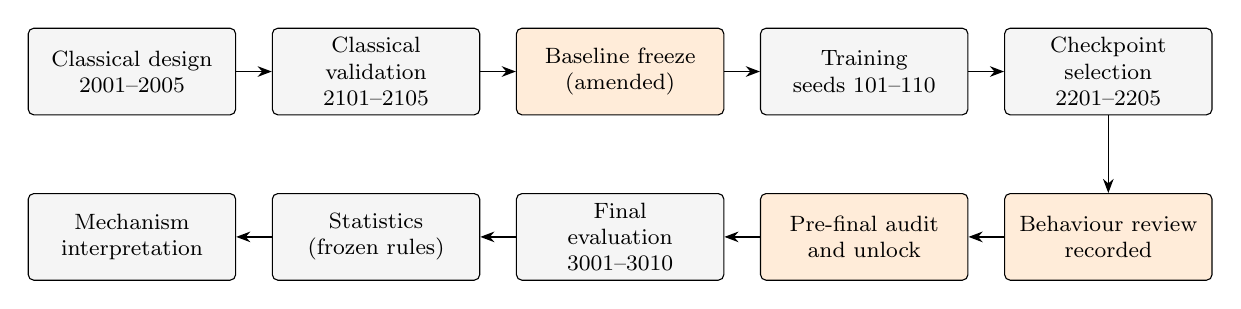
\begin{tikzpicture}[
  font=\footnotesize,
  st/.style={draw, rounded corners=2pt, align=center, fill=black!4, minimum height=11mm, text width=24mm},
  gate/.style={draw, rounded corners=2pt, align=center, fill=orange!15, minimum height=11mm, text width=24mm},
  ar/.style={-{Stealth[length=1.8mm]}, line width=0.5pt},
]
\node[st] (a) at (0,0) {Classical design\\2001--2005};
\node[st] (b) at (3.1,0) {Classical validation\\2101--2105};
\node[gate] (c) at (6.2,0) {Baseline freeze\\(amended)};
\node[st] (d) at (9.3,0) {Training\\seeds 101--110};
\node[st] (e) at (12.4,0) {Checkpoint selection\\2201--2205};
\node[gate] (f) at (12.4,-2.1) {Behaviour review\\recorded};
\node[gate] (g) at (9.3,-2.1) {Pre-final audit\\and unlock};
\node[st] (h) at (6.2,-2.1) {Final\\evaluation\\3001--3010};
\node[st] (i) at (3.1,-2.1) {Statistics\\(frozen rules)};
\node[st] (j) at (0,-2.1) {Mechanism\\interpretation};
\draw[ar] (a)--(b); \draw[ar] (b)--(c); \draw[ar] (c)--(d); \draw[ar] (d)--(e);
\draw[ar] (e)--(f); \draw[ar] (f)--(g); \draw[ar] (g)--(h); \draw[ar] (h)--(i); \draw[ar] (i)--(j);
\end{tikzpicture}}
\caption{Campaign order. Shaded stages are gates. Each stage requires
the verified completion record of every earlier stage, and each stage
may open only its own traffic family. The position of the behaviour
review relative to the unlock is described in
Section~\ref{subsec:behaviour}.}
\label{fig:protocol}
\end{figure}
% VERIFY: the frozen stage machine places learner validation (5) before
% the pre-final audit (6); confirm on which runs the behaviour review is
% computed and adjust the arrow f->g if needed.

\subsection{Training protocol}
\label{subsec:training}

Each learned method is trained once per training seed for exactly
360{,}000 joint transitions (1{,}800{,}000 simulated seconds of control
at 5~s per transition), giving 355{,}000 learner updates after the
5{,}000-transition warm-up. The budget is the same for all methods and
seeds, so comparisons are at matched interaction.
Each training episode uses a fresh manifest of the training family,
indexed by episode, and runs until the network clears, until the
7{,}200~s cap, or until the budget is exhausted. The final episode of a
run is normally cut short by the budget; this is a budget truncation,
not a clearance failure. Actions are $\varepsilon$-greedy with
independent random draws for the two agents
(Table~\ref{tab:hyperparameters}). Fourteen checkpoints are written at
the preregistered transition counts. Training outcomes (completion,
episodes, clearance events during training) are
\TBD{TBD_AFTER_LEARNER_TRAINING}.

\subsection{Checkpoint selection}
\label{subsec:checkpoint}

For every learned method and training seed, all fourteen checkpoints are
evaluated greedily ($\varepsilon=0$) on the five learner-validation
seeds. The selected checkpoint minimizes mean validation $\Jp$, then mean
validation time loss, then the transition count; the last tie-break
favours less training, which is the more conservative claim. Selection
never uses final-test traffic or the training episodes. Exactly one
checkpoint is selected per method and seed, giving ten selected policies
per method. Selected checkpoints: \TBD{TBD_AFTER_LEARNER_VALIDATION}.
% OPEN PROTOCOL ISSUE (must be resolved and documented BEFORE learner
% validation is run): the frozen selector requires finite validation
% J_primary and time loss for all 14 checkpoints and fails closed
% otherwise. A checkpoint whose validation run does not clear would make
% selection impossible for that seed. A precommitted rule is needed
% (e.g., a checkpoint with any non-clearing validation run is
% ineligible, and selection proceeds over eligible checkpoints; the
% ineligibility count is reported).

\subsection{Run validity}
\label{subsec:validity}

A run is admissible evidence only if all of the following hold: every
scheduled vehicle is accounted for; the status is cleared; no vehicle
disappears unexpectedly; no teleport or accounting error is unresolved;
the one-second evaluation log is complete; and all primary and required
secondary outcomes are finite. A run that fails any gate contributes no
value to any mean. In particular, $\Jp$ is never computed over the
vehicles that happened to finish, because that would reward a controller
in proportion to the vehicles it failed to serve. Non-finite values
cannot enter the statistical procedure, and the decision rule of
Section~\ref{subsec:decision_rules} requires every final-evaluation run
to be valid. Validity outcomes: \TBD{TBD_AFTER_FINAL_EVALUATION}.

\subsection{Behavioural review}
\label{subsec:behaviour}

A good network-average $\Jp$ can coexist with a starved movement or with
switching every interval. For every selected adaptive policy (each of
the ten QMIX, VDN and IDQN policies, canonical Max Pressure and P5), the
following distributions are reported per intersection and movement:
maximum and 95th-percentile service deprivation, the realized
green-duration distribution including the frequency and share of 2~s
greens, switch rate, yellow fraction of elapsed time, service frequency,
green share, 95th-percentile and maximum queue, the emergent-cycle
distribution, and clearance status. A movement's service deprivation is
the length of a maximal run of seconds in which that movement does not
show green, so it includes both the conflicting green and the yellow.
The emergent cycle is the interval between consecutive H-green starts at
the same intersection; it describes realized behaviour, not an imposed
cycle. The primary window is the demand period $[0,3600)$~s, and the
full episode up to clearance is reported as secondary information.
Switch counts and switch rates are defined only for controllers that
take online decisions; for pretimed plans they are reported as not
applicable rather than as zero. The review rule is
qualitative and fixed in advance: no pathological starvation or
flickering may be hidden by a good network-average $\Jp$. No numeric
threshold is defined, because a threshold chosen after the distributions
are seen would be fitted to them; the distributions are published in
full so that readers can apply their own. Each selected QMIX policy
receives its own recorded review, and the review is completed before any
paired performance comparison is computed. A review concluding
pathology for any selected QMIX policy makes a GO verdict impossible.
Comparator reviews are reported; comparator pathology never counts in
QMIX's favour. Reviews: \TBD{TBD_AFTER_LEARNER_VALIDATION}.
% VERIFY: state explicitly which runs (learner-validation runs of the
% selected checkpoints and/or final-test runs) feed the review, as
% implemented in the campaign scripts.

\subsection{Final evaluation}
\label{subsec:final_eval}

After the pre-final audit and the explicit unlock, every selected learned
policy is evaluated greedily on each of the ten final-test seeds, giving
a $10\times10$ matrix per learned method (training seed $\times$ traffic
seed). Each classical controller and P5 is deterministic given the
traffic and is evaluated once per final-test seed. All controllers meet
identical traffic at a given seed, and every comparison is paired within
seed. Final evaluation: \TBD{TBD_AFTER_FINAL_EVALUATION}.

\subsection{Statistical methodology}
\label{subsec:statistics}

For a treatment $T$ (QMIX) and a comparator $C$, the paired difference in
cell $(i,j)$, with training seed $i$ and final traffic seed $j$, is
\begin{equation}
D_{ij}=\Jp^{T}(i,j)-
\begin{cases}
\Jp^{C}(i,j) & \text{learned $C$ (same training seed $i$)},\\
\Jp^{C}(j) & \text{deterministic $C$}.
\end{cases}
\label{eq:difference}
\end{equation}
A deterministic comparator contributes one value per traffic seed and
is never treated as ten independently trained samples. The design is
crossed rather than nested: the same ten traffic seeds are used for
every training seed. The 95\% confidence interval of the mean difference
$\bar D$ is therefore obtained from a paired crossed two-factor
bootstrap. Each of 10{,}000 replicates resamples the ten training-seed
indices with replacement and, independently, the ten traffic-seed
indices with replacement. It then averages $D$ over the Cartesian
product of the two resamples, so that the same resampled traffic columns
apply to every resampled training row. The interval is the 2.5th--97.5th
percentile of the replicate means, and the bootstrap random-number
stream is fixed.
% TODO-LITERATURE: bootstrap methodology (Efron and Tibshirani) and a
% reference for bootstrapping crossed/two-way random-effects designs.
The training seed is the inferential unit for learning variability; the
100 cells are not treated as 100 independent replicates. The following
are also reported for each comparison:
the per-training-seed mean differences $\bar D_{i\cdot}$; the paired
effect size $d_z=\mathrm{mean}(\bar D_{i\cdot})/\mathrm{sd}(\bar D_{i\cdot})$;
the fraction of training seeds with $\bar D_{i\cdot}<0$; and the number
of training runs that completed under contract with a validly selected
checkpoint, with its Wilson score interval. The last quantity is a
property of the training process, never of performance.
% TODO-LITERATURE: Cohen's d_z for paired designs; Wilson (1927) score
% interval.

\subsection{Decision rules and precommitted interpretations}
\label{subsec:decision_rules}

The decision rules (protocol \texttt{go-no-go-1.1}) were fixed and
hashed before any learner-validation or final-test result existed and
before any learner result was admitted to inference (Table~\ref{tab:decision}). The qualification outcome is
GO if and only if all four conditions hold:
\begin{enumerate*}[label=(\roman*)]
\item the 95\% interval for $\Jp^{\mathrm{QMIX}}-\Jp^{\mathrm{OFT}}$ lies
entirely below zero, where OFT denotes optimized fixed timing;
\item the 95\% interval for $\Jp^{\mathrm{QMIX}}-\Jp^{\mathrm{IDQN}}$
lies entirely below zero;
\item every hard validity gate passes;
\item every selected QMIX policy has a completed behavioural review and
none concludes pathology.
\end{enumerate*}
No minimum effect size is required and none may be introduced after the
results are seen; effect sizes are reported so that practical relevance
can be judged. The comparisons with VDN, canonical Max Pressure and P5
are reported with their intervals but do not decide.

\begin{table}[!htbp]
\centering
\caption{Preregistered comparisons (protocol \texttt{go-no-go-1.1}).}
\label{tab:decision}
\small
\begin{tabularx}{\textwidth}{@{}L{4.4cm}L{2.6cm}Y@{}}
\toprule
Comparison & Role & Question \\
\midrule
QMIX $-$ optimized fixed timing & deciding & Does adaptive control beat the best pretimed plan found by the same search budget? \\
QMIX $-$ IDQN & deciding & Does cooperative value decomposition add to independent learning? \\
QMIX $-$ VDN & reported & Does the monotonic mixer add to additive decomposition? \\
QMIX $-$ canonical Max Pressure & reported (mandatory) & How does QMIX compare with a strong operational adaptive controller? \\
QMIX $-$ P5 & diagnostic & Pressure logic versus learned policy under equal authority. \\
\bottomrule
\end{tabularx}
\end{table}

The interpretations of the possible outcomes were also fixed in advance:
\begin{description}[leftmargin=1.2cm,style=nextline]
\item[Case A] QMIX beats IDQN but not optimized fixed timing:
cooperative value factorization improves on independent adaptive
learning, but a carefully optimized pretimed plan remains competitive at
this operating point. The primary gate fails.
\item[Case B] QMIX beats optimized fixed timing but not VDN: adaptive
control is beneficial, but additive decomposition appears sufficient for
two agents. No claim of superiority of the QMIX architecture is made.
\item[Case C] QMIX beats the learning baselines but not canonical Max
Pressure: learned coordination improves on the learning baselines, but a
traffic-structured pressure controller remains operationally stronger in
this regime. This is reported prominently.
\item[Case D] QMIX attains a good $\Jp$ with pathological starvation or
flickering: the improvement is not operationally acceptable under the
unconstrained authority, and the verdict is a behavioural NO-GO.
\end{description}
Outcome: \TBD{TBD_AFTER_FINAL_EVALUATION}.

\subsection{Mechanism and coordination analysis}
\label{subsec:mechanism}

Whether the two learned agents coordinate is treated as an empirical
question, answered only from logged behaviour. The following diagnostics
were preregistered and are computed for each direction of travel on the
central link, WE (J1 to J2) and EW (J2 to J1):
\begin{itemize}
\item \emph{phase cross-correlation} $\rho(\ell)=\mathrm{corr}\bigl(g_1(t),g_2(t+\ell)\bigr)$
between the H-green indicators of J1 and J2, for lags $|\ell|\leq120$~s,
where a positive lag means that J2 follows J1;
\item the \emph{green-start lag distribution}, the time from each H-green
start at one intersection to the next H-green start at the other;
\item \emph{green at approach detector} (GAD50), the fraction of vehicle
crossings of a virtual detector 50~m upstream of the downstream stop
line, at 229.2~m along the 279.2~m central lane, that occur while the
downstream H phase is green;
\item a \emph{projected arrival-on-green} proxy obtained by projecting
detector crossings to the stop line at free-flow speed. It is labelled
as a projection and never reported as an observed arrival-on-green;
\item \emph{downstream stops} of vehicles on the central link.
\end{itemize}
Time-resolved versions use 300~s windows advanced in 60~s steps. All
travel-time reasoning uses the simulated 279.2~m lane length. Because
the learned controllers can shift their phase changes relative to each
other only in 5~s steps (Section~\ref{subsec:executor}), a lag structure
is interpreted at that resolution. These diagnostics describe behaviour;
by themselves they do not establish that coordination causes any
difference in $\Jp$. Results: \TBD{TBD_AFTER_FINAL_EVALUATION}.
% TODO-LITERATURE: arrival-on-green / Purdue coordination diagram
% references for GAD50 and projected AOG.

\subsection{Optional high-demand robustness slice}
\label{subsec:robustness}

\TBD{OPTIONAL_ROBUSTNESS_AFTER_PRIMARY_GATE}.
If carried out, the selected policies and plans would be evaluated
without retraining or re-optimization at demand multipliers
$\rho\in\{1.5,2.0\}$, keeping the 300~m nominal spacing. A binary
reporting rule is fixed in advance: if QMIX fails to clear at a demand
level at which optimized fixed timing clears under the same evaluation
protocol, this is reported as a QMIX generalization failure at that
level. This slice is not part of the primary decision and may be
omitted from the main paper.

\subsection{Reproducibility and provenance}
\label{subsec:provenance}

All official runs execute from a clean checkout of a single frozen
source commit. Every run records the commit, the working-tree status,
the hashes of the configuration, network, traffic manifest and route
file, the SUMO seed, and the software versions (Python~3.7.16,
NumPy~1.21.6, PyTorch~1.13.1 on CPU, SUMO~1.25.0). A completed run
carries a hash-sealed completion record; a run is reused only if that
record, its metrics and its environment identity all verify. Stage
completion records and the baseline freeze are hash-sealed, not
cryptographically signed. Table~\ref{tab:provenance} lists the frozen
identities.

\begin{table}[!htbp]
\centering
\caption{Frozen identities (SHA-256 unless stated).}
\label{tab:provenance}
\scriptsize
\begin{tabularx}{\textwidth}{@{}L{4.0cm}Y@{}}
\toprule
Item & Identity \\
\midrule
Source commit (Git) & \texttt{8c14f32988e92ddc6b1421d70258f5fbd2f2cc4d} \\
Adaptive configuration & \texttt{18342d3b6e9646d062f63ebc8474571cdedb151c49bbe50b375130ff98f7c954} \\
Baseline configuration & \texttt{c25393bb5bfd4ab03d8f0527fb15fe1037d04cf75795d8550ea8e0361d21ef4a} \\
Network file & \texttt{3f4449c40fb6497fd6605da14246ef09432c74327f21b23a0984b0e2f1f5a790} \\
Primary control specification & \texttt{32bb79d159eacf7693462338d366715dad0fa494a4b619667aec818ba7c21841} \\
Decision protocol \texttt{go-no-go-1.1} & \texttt{de724720e131cc5f6a72191c7b6d4e87a77223a83ae21cec58a40b530f743f21} \\
Statistical protocol \texttt{statistics-1.1} & \texttt{72769a92394ccd79d7712690a3f93413e3955dea100a823436bd0bff727777cf} \\
Protocol Amendment 001 & \texttt{edb9ec98281b6a9588fae96cfdf982eb90984b830b7fa815ad058160b3ba020a} \\
Protocol Amendment 002 (sealed addendum and driver) & \TBD{TBD_AFTER_FINALISE_COARSE} \\
Amended baseline freeze & \TBD{TBD_AFTER_TIMING_VALIDATION} \\
\bottomrule
\end{tabularx}
\end{table}
% The configuration and protocol hashes above were computed from the
% frozen commit with its own hashing functions; re-verify against the
% freeze artefacts before submission.

\paragraph{Chronology and deviations} The protocol was amended twice,
and the relation of each amendment to existing evidence is stated
explicitly.
Amendment 001 was documented after one official QMIX training run (seed
101) had already been launched; the lower-cycle audit simulations were
run after the amendment.
Amendment 002 was finalized and sealed before the structural-floor and
reopened fine-search simulations. The lower-cycle evidence it reuses
already existed and was reused only after explicit provenance checks and
realized-plan equivalence checks. No result of that run was used for any
baseline decision, no checkpoint had been selected, and neither the
learner-validation nor the final-test family had been accessed. As
Amendment 001 precommitted for the case that the fixed-timing track was
reopened, that run is treated as pre-amendment engineering evidence: it
is excluded from inference, and seed 101 is trained again under the
amended freeze. Because training is configured to be deterministic, the
checkpoint hashes of the two seed-101 runs are compared and reported:
\TBD{TBD_AFTER_LEARNER_TRAINING}. A first draft of Amendment 002 was
withdrawn before execution because it identified candidates by
parameter labels rather than by the executed plan; it is archived with
its hashes.

% =====================================================================
\section{Results}
\label{sec:results}
% =====================================================================
% SKELETON ONLY. The order below follows the gate order: validity and
% behaviour are reported before any performance comparison.

\subsection{Selected classical baselines}
\label{subsec:res_baselines}
\paragraph{Combined coarse ranking} The combined coarse ranking over
the original, lower-cycle and structural-floor grids produced the five
best realized plans listed in Table~\ref{tab:coarse_top5}. Their
design-set scores are selection-optimistic, because these plans were
retained for scoring best on the design seeds. They are therefore not
estimates of baseline performance and are given only in the Supplement.
The 5~s classical minimum green is active, on the side-street green, in
the three best plans. The structural floor $C=16$~s was evaluated and
did not produce a top-five plan.

\begin{table}[!htbp]
\centering
\caption{Five best realized plans of the combined coarse ranking (design
seeds 2001--2005). Rank order only; these are not the selected baseline.}
\label{tab:coarse_top5}
\small
\begin{tabularx}{\textwidth}{@{}cL{3.6cm}L{4.2cm}Y@{}}
\toprule
Rank & Realized $(C,g_H,g_V,\Delta)$ (s) & Coarse labels $(C,1000f_H,\Delta)$ & Active constraints \\
\midrule
1 & (18, 7, 5, 10) & (18, 550, 10), (18, 600, 10) & $g_V=5$ \\
2 & (19, 8, 5, 10) & (19, 600, 10), (19, 650, 10) & $g_V=5$ \\
3 & (20, 9, 5, 10) & (20, 650, 10) & $g_V=5$ \\
4 & (25, 12, 7, 0) & (25, 650, 0) & none \\
5 & (25, 13, 6, 0) & (25, 700, 0) & none \\
\bottomrule
\end{tabularx}
\end{table}
% Aliases derived from the frozen combined coarse grid and checked; the
% fine-union counts (1,359 labels -> 792 plans) were independently
% recomputed from the frozen grids and match the finalise-coarse output.

\paragraph{Fine search} The union-of-aliases fine search around these
five plans comprises 1{,}359 labels and 792 realized plans. Design runs
already existed for 87 of them, so 705 new plans (3{,}525 new design
runs) are required. The ten best then proceed to 50 validation runs.

\paragraph{Selected plan} \TBD{TBD_AFTER_TIMING_VALIDATION}. Held-out
performance of the selected plan is reported only in
Section~\ref{subsec:res_primary}.

\subsection{Training and checkpoint selection}
\label{subsec:res_training}
Training completion, training-success count with Wilson interval, and
the selected checkpoint per method and seed:
\TBD{TBD_AFTER_LEARNER_TRAINING}; \TBD{TBD_AFTER_LEARNER_VALIDATION}.

\subsection{Validity and behavioural review}
\label{subsec:res_behaviour}
Validity gates for all final-evaluation runs, and the behavioural
distributions and recorded review for every selected adaptive policy:
\TBD{TBD_AFTER_FINAL_EVALUATION}.
% Planned table: per method, median and range across training seeds of
% switch rate, yellow fraction, share of 2 s greens, p95/max service
% deprivation per movement, green share, emergent-cycle quantiles.
% Planned figure: green-duration distributions (QMIX, VDN, IDQN, MP, P5).

\subsection{Primary outcome}
\label{subsec:res_primary}
$\Jp$ for all controllers on the final-test seeds, and the two deciding
comparisons with their crossed 95\% intervals, $d_z$ and the fraction of
training seeds favouring QMIX: \TBD{TBD_AFTER_FINAL_EVALUATION}.
% Planned table: mean and sd of J_primary per controller; for each
% comparison of Table 7: mean difference, 95% CI, d_z, fraction of seeds.
% Planned figure: per-training-seed mean differences with the crossed CI.

\subsection{Reported comparisons: VDN, Max Pressure and P5}
\label{subsec:res_reported}
\TBD{TBD_AFTER_FINAL_EVALUATION}.

\subsection{Secondary outcomes}
\label{subsec:res_secondary}
\TBD{TBD_AFTER_FINAL_EVALUATION}.

\subsection{Mechanism and coordination diagnostics}
\label{subsec:res_mechanism}
\TBD{TBD_AFTER_FINAL_EVALUATION}.

\subsection{High-demand robustness slice}
\label{subsec:res_robustness}
\TBD{OPTIONAL_ROBUSTNESS_AFTER_PRIMARY_GATE}.

% =====================================================================
\section{Discussion}
\label{sec:discussion}
% =====================================================================
% SKELETON ONLY. Each subsection is written from the final evidence and
% from the precommitted interpretation (Cases A--D) that applies.

\subsection{What short-interval authority buys}
\TBD{TBD_AFTER_FINAL_EVALUATION}.
% Separate (i) learned vs pressure logic under equal authority (QMIX vs
% P5), (ii) authority itself (P5 vs canonical MP), (iii) adaptive vs
% optimized pretimed (QMIX vs OFT). Do not attribute a J difference to
% coordination unless the diagnostics of subsec:res_mechanism support it.

\subsection{Cooperation and the mixer}
\TBD{TBD_AFTER_FINAL_EVALUATION}.

\subsection{Interpreting the optimized pretimed plan}
\TBD{TBD_AFTER_TIMING_VALIDATION}.
% Established at finalise-coarse (result-independent of learners): the 5 s
% classical minimum green is active (g_V = 5 s) in the three best coarse
% plans, so the best pretimed plans sit on the admissibility boundary for
% the side-street green. The comparison with the learned controllers,
% which may use 2 s greens, must be discussed with this in mind.
% TODO-LITERATURE (required before submission): external source for the
% 5 s classical minimum green.
% If the selected plan has a short cycle, discuss it as a rapid-service
% plan unless the coordination diagnostics support a progression
% interpretation. Webster may be cited as background only; no numerical
% Webster cycle is computed without measured saturation flows.

\subsection{Operational acceptability}
\TBD{TBD_AFTER_FINAL_EVALUATION}.
% Short greens, switching burden, yellow fraction, service deprivation;
% relation to practical minimum greens and pedestrian requirements, which
% this study does not model.

% =====================================================================
\section{Limitations}
\label{sec:limitations}
% =====================================================================
% Result-independent limitations are drafted; result-dependent ones are
% marked.

\paragraph{Scope} The evidence concerns one synthetic corridor with two
intersections, one nominal spacing, one steady demand level and through
movements only. No claim is made for larger networks, other spacings,
time-varying demand or turning movements.

\paragraph{Simulation fidelity} SUMO's car-following and insertion
models, perfect and noise-free detection through TraCI, and the absence
of pedestrians and of detector failures all separate the simulated
controller from a deployed one.

\paragraph{Asymmetric control constraints} The learned controllers may
produce 2~s greens and have no minimum green, whereas pretimed plans
must keep greens of at least 5~s and canonical Max Pressure at least
10~s. In the other direction, the learned controllers act on a
synchronized 5~s grid, while pretimed offsets are set at 1~s
resolution. The comparison is therefore between controllers with
different, explicitly stated authorities, not with matched constraints.
The 5~s classical minimum green is active in the three best coarse
plans, so the pretimed optimum is constrained by a rule that the learned
controllers do not face.
% TODO-LITERATURE (required before submission): external source for the
% 5 s classical minimum green.
P5 isolates part of this difference.

\paragraph{Search resolution of the pretimed baseline} Coarse cycles
are searched on a 5~s lattice, extended down to the 16~s structural
minimum, and fine cycles in 5~s steps around each centre. Plans between
lattice points are not evaluated. In particular, $C=17$~s was evaluated
only at coarse offset resolution ($\Delta\in\{0,5,10,15\}$~s). The
preregistered fine rule, with 5~s cycle steps and the clip $[16,140]$~s,
does not revisit it from the centres that were retained; the same holds
for $C=16$~s. The design-set scores differ markedly between adjacent
cycles among the best plans, so the landscape is not smooth at this
resolution, and an unevaluated cycle could score differently from its
neighbours. The design scores of the retained candidates are
selection-optimistic, which is why selection uses separate validation
traffic and performance is reported only on held-out traffic.

\paragraph{Outcome definition} $\Jp$ counts time at or below 0.1~m/s and
insertion delay, not slowdowns above that speed; time loss is therefore
reported alongside it. Conclusions refer to $\Jp$ as defined.

\paragraph{Learning configuration} All learned methods share one frozen
configuration that was not tuned separately for each method; a
different configuration could change their relative performance. Ten
training seeds bound the precision of learning-variability estimates.

\paragraph{Result-dependent limitations} \TBD{TBD_AFTER_FINAL_EVALUATION}.

% =====================================================================
\section{Conclusion}
\label{sec:conclusion}
% =====================================================================
\TBD{TBD_AFTER_FINAL_EVALUATION}.

% =====================================================================
\section*{Code and Data Availability}
% =====================================================================
The source code at the frozen commit, the SUMO network, the traffic
manifest generator, controller implementations, protocol amendments,
analysis scripts and the seed-level data needed to reproduce every
reported statistic will be released in a public archive upon
acceptance. \TBD{TBD_AFTER_FINAL_EVALUATION}: archive identifier and
checkpoint manifest with hashes.

\section*{CRediT Authorship Contribution Statement}
\textbf{Mohamed Yassine Neifar:} Conceptualization, Methodology, Software, Validation, Formal analysis, Investigation, Data curation, Visualization, Writing -- original draft, Writing -- review and editing.
\textbf{Nadir Farhi:} Conceptualization, Methodology, Validation, Supervision, Writing -- review and editing.
\textbf{Ahmed Frikha:} Supervision, Writing -- review and editing.
% VERIFY contributions for the new study with all authors.

\section*{Funding}
This research did not receive any specific grant from funding agencies in the public, commercial, or not-for-profit sectors.

\section*{Declaration of Competing Interest}
The authors declare that they have no known competing financial interests or personal relationships that could have appeared to influence the work reported in this paper.

\section*{Declaration of Generative AI and AI-Assisted Technologies in the Writing Process}
During the preparation of this work, the authors used AI-assisted tools
to support code review, manuscript organization, language editing and
consistency checking. After using these tools, the authors
independently verified the scientific statements, calculations,
citations, code outputs and reported results, reviewed and edited the
content as needed, and take full responsibility for the content of the
published article.
% VERIFY: name the tools actually used, as in the journal's policy.

\section*{Acknowledgements}
The authors acknowledge the academic guidance and scientific support provided within the doctoral research collaboration between the University of Sfax and Universit\'e Gustave Eiffel.

\bibliographystyle{elsarticle-num}
\bibliography{References}

\end{document}
